\begin{figure}[h!]
	\centering
	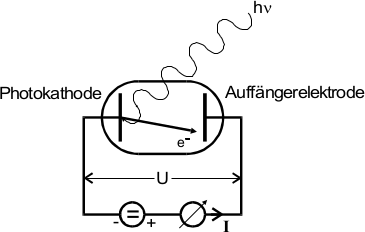
\includegraphics[width=0.4\textwidth]{SchematischerAufbau.png}
	\caption{Schematische Versuchsanordnung zur Beobachtung des Photoeffekts \cite{\V}}
	\label{fig:schematischerAufbau}
\end{figure}
Um den Photoeffekt beobachten zu können kann ein Versuchsaufbau, wie er in Abbildung \ref{fig:schematischerAufbau} dargestellt ist verwendet werden. Das Licht überträgt seine Energie auf die Elektronen in der Photokathode. Ist diese Energie mindestens so groß, wie die Austrittsarbeit $A_\text{K}$, werden Elektronen ausgelöst und bewegen sich in Richtung Auffängerelektrode, wo sie mit dem Ampère-Meter als (Photo-)Strom gemessen werden können. Die Beschleunigungsspannung $U$ zwischen den beiden Elektroden ist variabel. Nur wenn ein Elektron nach dem Austritt eine kinetische Energie von mindestens
\begin{align}
	E_ = \frac{1}{2}mv^2 = eU \ ,
\end{align}
mit der Elementarladung $e$, hat, kann es die Auffängerelektrode erreichen und als Strom detektiert werden. Die Spannung, bei der gerade keine Elektronen mehr die Auffängerelektrode erreichen heißt Grenzspannung $U_\text{g}$ und ist ein Maß für die maximale kinetische Energie der ausgelösten Elektronen (Photoelektronen)
\begin{align}
	E_\text{max} = eU_\text{g} \ .
\end{align}
Der Photostrom beschreibt die Anzahl der Photoelektronen pro Zeit. \\
Das Wellenmodell des Lichts suggeriert folgendes Verhalten: Die Elektronen an der Metalloberfläche werden durch das elektrische Feld des Lichts zu erzwungenen Schwingungen angeregt. Wenn die Schwingungsamplitude groß genug ist, können die Elektronen aus dem Metall austreten. Das bedeutet für die Erwartung an die Messung:
\begin{itemize}
	\item Aufgrund von Resonanzphänomenen muss der Photostrom bei Lichtfrequenzen, die den Resonanzfrequenzen der Elektronen entsprechen, besonders hoch sein.
	\item Die Intensität beschreibt die Energie pro Zeit und Fläche. Daher sorgt sehr intensives Licht für sehr energiereiche Elektronen.
	\item Auch bei sehr langwelligem Licht mit hoher Intensität werden Elektronen ausgelöst.
\end{itemize}
Die tatsächlichen Beobachtungen widersprechen diesen Erwartungen:
\begin{itemize}
	\item Der Photostrom ist proportional zur Lichtintensität.
	\item Die kinetische Energie der Photoelektronen ist proportional zur Lichtfrequenz und unabhängig von der Intensität.
	\item Es existiert eine Grenzfrequenz, unterhalb der der Photoeffekt nicht auftritt. Andere ausgezeichnete Frequenzen existieren nicht.
\end{itemize}
Aus der Wellenbeschreibung des Lichts folgt, dass die Energie der Strahlung gleichmäßig und proportional zur Intensität verteilt ist. Dem Experiment zufolge beschreibt eine Welle das Licht aber nur unzureichend. Einsteins Vorschlag lautete also:
\par
\begingroup
\leftskip1.5cm
\rightskip\leftskip
{Licht besteht aus räumlich verschwindend kleinen Teilchen, den Photonen. Sie bewegen sich mit der Lichtgeschwindigkeit $c$ und transportieren die Energie in diskreten Mengen, mit dem Wert $E=h\nu$. Dabei ist $\nu$ die Lichtfrequenz und $h$ das Plancksche Wirkungsquantum.}
\par
\endgroup
Der Photoeffekt lässt sich damit gut erklären: Die Photonen bewegen sich auf das Metall zu. Dort stößt ein Photon mit genau einem Elektron und gibt seine gesamte Energie ab. Wenn gilt
\[ h\nu > A_\text{K} \ ,\]
verwendet das Elektron einen Teil der ihm übertragenen Energie zum Austritt aus der Metalloberfläche. Der andere Teil geht über in seine kinetische Energie
\begin{align}\label{eq:einstein}
	E = h\nu - A_\text{K} \ .
\end{align}
Gleichung \ref{eq:einstein} wird auch Einstein-Gleichung genannt \cite{Gerthsen}. \\
Die Frequenz $\nu_\text{g}$, für die gilt
\[ h\nu_\text{g} = A_\text{K} \ , \]
wird Grenzfrequenz genannt. Bei jeder Frequenz $\nu<\nu_\text{g}$ ist die Energie des Photons kleiner als die Austrittsarbeit. Das heißt kein Elektron kann das Metall mehr verlassen, es tritt kein Photoeffekt auf.